% \documentclass[letterpaper,twocolumn,10pt]{article}
% \usepackage{usenix,epsfig,endnotes}

\documentclass[letterpaper,10pt,twocolumn]{article}
\usepackage{epsfig}
\usepackage{subfigure}
\usepackage{xspace}
\usepackage{amsmath}
% One inch margins all around for letter-size paper:
\oddsidemargin 0in
\evensidemargin 0in
\topmargin -.5in
\textwidth 6.7in
\textheight 9.1in

% \usepackage{enumitem}
% \setitemize{noitemsep,topsep=0pt,parsep=0pt,partopsep=0pt}

\newcommand{\sub}{subquorum\xspace}
\newcommand{\Sub}{Subquorum\xspace}
\newcommand{\subs}{subquorums\xspace}
\newcommand{\Subs}{Subquorums\xspace}
\newcommand{\sys}{Alia\xspace}
\newcommand{\roo}{root quorum\xspace}
\newcommand{\roos}{root quorums\xspace}
\newcommand{\Roo}{Root quorum\xspace}
\newcommand{\Roos}{Root quorums\xspace}
\newcommand{\para}[1]{\vspace{.04in}\noindent\textbf{#1}}

\newcommand{\hmm}[1]{}%{#}1

\newcommand{\dspace}{\renewcommand{\baselinestretch}{.985}\Large\normalsize}

\dspace

% Pete's editing special sauce
\usepackage[usenames,dvipsnames,svgnames,table]{xcolor}
\newcommand{\todo}[1]{{\textcolor{red}{#1}}}
\newcommand{\pjk}[1]{{\textcolor{red}{PJK: #1}}}
\newcommand{\ben}[1]{{\textcolor{orange}{Ben: #1}}}


\def\mcn#1{\multicolumn{1}{c}{#1}}
\def\mc#1{\multicolumn{1}{|c|}{#1}}
\def\mcl#1{\multicolumn{1}{||c|}{#1}}
\def\mclr#1{\multicolumn{1}{||c||}{#1}}
\def\mcr#1{\multicolumn{1}{|c||}{#1}}
\def\mctwo#1{\multicolumn{2}{|c|}{#1}}
\def\tmcr#1{\multicolumn{2}{|c||}{#1}}
\def\mcthree#1{\multicolumn{3}{|c|}{#1}}
\def\mcthreer#1{\multicolumn{3}{|c||}{#1}}
\def\mcfour#1{\multicolumn{4}{|c|}{#1}}
\def\mcfourr#1{\multicolumn{4}{|c||}{#1}}
\def\mcfive#1{\multicolumn{5}{|c|}{#1}}
\def\mcfiver#1{\multicolumn{5}{|c||}{#1}}
\def\mcsix#1{\multicolumn{6}{|c|}{#1}}
\def\mcsixr#1{\multicolumn{6}{|c||}{#1}}
\def\mcseven#1{\multicolumn{7}{|c|}{#1}}
\def\mcsevenr#1{\multicolumn{7}{|c||}{#1}}
\def\rot#1{\begin{sideways}#1\end{sideways}}
\def\lb#1{\raisebox{-1.5ex}[0em][0em]{#1}}
\def\rb#1{\raisebox{1.5ex}[0em][0em]{#1}}
\def\hdg#1{\vspace{0.1in}\noindent{\bf #1}\\}

\begin{document}

%don't want date printed
\date{}

%make title bold and 14 pt font (Latex default is non-bold, 16 pt)
\title{\Large \bf There Is More Consensus in the Hierarchy }

% \authorinfo{Benjamin Bengfort}
%            {University of Maryland}
%            {bengfort@cs.umd.edu}
% \authorinfo{Pete Keleher}
%            {University of Maryland}
%            {keleher@cs.umd.edu}

\author{\emph{Omitted for review}}
% \author{\rm{Benjamin Bengfort} and \rm{Pete Keleher}\\
% University of Maryland, College Park\\
% \{bengfort,keleher\}@cs.umd.edu}

\maketitle

% Use the following at camera-ready time to suppress page numbers.
% Comment it out when you first submit the paper for review.
\thispagestyle{empty}

\hmm{
triple:   <epoch,qid,term> describes leader

new epoch, replicas need to archive old log, clean slate new log

log



subs
- commit announcement
- updated ids
- truncate
- insert announcement
- start

- wait for tombstone, and root

Notes:
- focus on edges and putting them together.
- to what extent are we altering the basic protocol?


In what way are we modifying the basic protocol?
- The biggest change to the original protocol is the inclusion of the epoch number - this influences every Raft invariant. E.g. where there was a term check before, now there is a term/epoch check. This is the only change at the subquorum level I can think of right now.
- heartbeats
- reqs AND resps must have sub id and rep id
- no leader
- two related states: root and sub (even if not currently assigned to sub)
- logs truncated upon moving into new epoch. This is necessary because new epoch might
  pair reps different reps (have different old logs)
- root
  - different heartbeats
  - delegation
  - multiple personas (logs, participation)
    - what is needed to make multiple logs work?
       - (tables/msgs augmented with persona ids?)
    - At a higher level, how is this different than distinct replicas?
      - What are the advantages?

I'm thinking serious of folding alia back into the hier section.
- We'd need to have a "lessons learned" list
  - fuzzy transitions important for avoiding lockstep (though we can't
show this)
  - bilateral (vs global) handshakes across remapping
  - it's not the size of the quorum, it's the cost of waiting for the
important ones

``Delegation'' is a silver bullet for nuclear option.  ``Consider without
delegation....multiple leaders elected....''

Approaches:
1) pull data on-demand (reads slow for quite a while)
2) log replication (much useless stuff, old versions, things not caring for.
3) suffix of log to accounts to leverage locality

- How to even find the logs? We have announcements, can walk backwards.
- logs reflect an overlapping, but possibly not identical tag

Pull current version of database through combination of background anti-entropy, demand
requests, and transition-initiated pull, leader-to-leader. Old versions are not pulled, as
they are backed up in logs.


}

\subsection*{Abstract}

We introduce \emph{Hierarchical Consensus} (HC), a new approach to generalizing and
localizing distributed consensus.
HC is well-suited for large, dynamic, and geo-replicated groups of hosts.
Hierarchical Consensus uses partitions among multiple \subs to increase
overall availability, localize decision-making, and improve throughput.

The key novelty is in allowing multiple decision-making \subs to run
independently.
\Subs can be lightweight, and chosen from hosts with low mutual communication
latencies.
Multiple independent \subs increase the system's overall throughput, while
their small sizes and co-location allow them to reach decisions quickly.
A \roo maintains the decision-space partition and provides linearizable
guarantees across the entire system.
We demonstrate HC's advantages through an implementation running on Amazon
EC2.

\section{Introduction}
Solutions to distributed consensus generally require high throughput, low latency, fault
tolerance, and durability.
Current
approaches~\cite{biely_s-paxos:_2012,mao_mencius:_2008,moraru_there_2013,kraska_mdcc:_2013,shapiroConsensus}
usually assume a small number of replicas in a co-located consensus group, each centrally
located on a highly available, powerful, and reliable host.
These assumptions are justified by the environments in which they usually run: highly
curated environments of individual data centers, centers connected by dedicated
networks, or dedicated clusters.

We consider the problem of using distributed consensus to support linearizable access
orderings for objects stores or global file systems.
Our target environments include geo-replicated machines across the Internet with no guarantees on
bandwidth, latency, or lack of partitions.
We further wish to accommodate replicas with heterogeneous capabilities and
usage modalities, such as systems including both highly-provisioned servers and
mobile devices.
This problem space is important, as it encompasses a wide variety of usages, from
agglomerations of the environments assumed by previous systems down to ad hoc
systems of local and personal devices.

This wider environment poses several new challenges.
Widely distributed replicas might have neither high bandwidth nor low latency, and might
suffer partitions of varying durations.
Such systems of replicas might also be dynamic in membership, in relative
location, and in workload.
Straightforward approaches to running variants of
Paxos~\cite{lamport_paxos_2001} or Raft~\cite{raft} across the wide area will perform
poorly for several reasons.
First, distance (in network connectivity) between consensus replicas and the
most active replicas decreases the performance of the entire system.
Second, network partitions in such an environment are common, either through
widespread network disruption or because active devices are carried into
an area of low reception.
Finally, since we do not assume that the replicas running consensus are
highly curated, the fault tolerance of a potentially large system can be
disrupted by a very small number of unreliable hosts.
Despite these issues, geo-replicating systems can be crucial for fault-tolerance, access to
resources, and supporting mobility.

We propose another approach to building large systems.
Rather than relying on a few replicas to provide consensus to many clients, we
propose to run a consensus protocol across replicas running at or near all of
those locations.
The key insight of this work is that \emph{large problem spaces can often be partitioned
into mostly disjoint sets of activity without violating consistency}.
We exploit this decomposition property by making our consensus protocol hierarchical, and
individual consensus groups fast by ensuring they are small.
We exploit locality by building \subs from co-located replicas, and locating \subs near
clients they serve.

Our main contributions are the following:
\begin{itemize}
\item We describe Hierarchical Consensus, a two-tiered consensus
  structure that allows high throughput, localization,
  agility, and linearizable access to a shared namespace.
\item We show how to use \emph{delegation} to build large consensus
groups that retain their fault tolerance properties while
performing like small groups.
\item We describe the use of \emph{fuzzy epoch transitions} to allow
  global re-configurations across multiple consensus groups without
  forcing them into lockstep.
\item We build a linearizable key-value store whose consensus group
  makeup and object namespace can be rapidly re-assigned across the
  entire group.
\item We build a sequentially-consistent replicated log from
  geo-replicated \sub logs.
\end{itemize}
The challenge is in building a multi-group coordination protocol that
configures and mediates the \subs through a \roo.
The \roo guarantees correctness by pivoting the overall system through two
primary functions.
First, the \roo re-configures \sub memberships on replica failures and
system membership changes.
Second, the \roo adjusts the mapping of the object namespace to the underlying partitions.
Much of the system's complexity comes from handshaking between the \roo and the
lower-level \subs during re-configurations.

These handshakes are made easier, and much more efficient, by using
\emph{fuzzy transitions}.
Fuzzy transitions allow individual \subs to move through re-configurations at
their own pace.
Given our heterogeneous, wide-area environment, forcing the entire system to
transition to new configurations in lockstep would be unacceptably slow.

% Enabled usage situation:
% \begin{itemize}
% \item multiple sets of homogeneous replicas from distinct clusters or data centers
% \item random set of replicas from across the Internet
% \item collections of ad hoc collections of personal or company-wide devices
% \end{itemize}
%
% Systems to be built on this mechanism include:
% \begin{itemize}
% \item key-value stores
% \item resource management
% \item global file systems
% \end{itemize}

We validate our approach by using HC to build \sys, a
linearizable~\cite{linearizability,attiya_sequential_1994} object
store explicitly intended to run with many replicas,
geo-replicated across heterogeneous networks and devices.
The resulting system is local, in that replicas serving clients can be
located near them.
The system is fast because individual operations are served by small
groups of replicas, regardless of the size of the total system.
The system is nimble, in that it can dynamically re-configure the
number, membership and responsibilities of \subs in response to
failures, phase changes in the driving applications, or mobility among
the member replicas.
Finally, the system is consistent, supporting the strongest form of
per-object consistency without relying on special-purpose
hardware~\cite{fawn,corfu,tango,spanner,vcorfu} or server farms.



The remainder of the paper presents the HC protocol (Section~\ref{sec:protocol}),
describes our implementation (Section~\ref{sec:implementation}), evaluates HC
(Section~\ref{sec:evaluation}), discusses related work (Section~\ref{sec:related}), and
concludes (Section~\ref{sec:conclusions}).

\section{Background}
\label{sec:background}

The canonical distributed consensus used by systems today is
Paxos~\cite{paxos,lamport_paxos_2001}.
Paxos is provably safe and designed to make progress even when a portion of
the system fails.
Raft~\cite{raft} was designed not to improve performance, but to increase
understanding of consensus behavior to better allow efficient implementations.
HC uses Raft as a building block, so we describe the relevant portions of Raft
at a high level, referring the reader to the original paper for complete details.

\para{Raft:}
Consensus protocols typically have two phases: leader
\emph{election} and operations \emph{commit}\footnote{Election and commit
  phases correspond to PROPOSE and ACCEPT phases in Paxos.}.
Raft is a strong-leader consensus protocol, which allows the election
phase to be elided while a leader remains available.
The protocol requires only a single communication round to commit an
operation in the common case.
Raft uses timeouts to trigger phase changes and provide fault
tolerance.
Crucially, it relies on timeouts only to provide progress, not safety.
New elections occur when another replica in the quorum
times out waiting for communication from the leader.
Such a replica increments its \emph{term} until it is greater than the
existing leader, and announce its candidacy.
Other replicas vote for the candidate if they have not seen a competing
candidate with a larger term.
During regular operation, clients send requests to the leader, which
broadcasts \texttt{AppendEntries} messages carrying
operations to all replicas.
An operation is \emph{committed} and can be executed when the leader
receives acknowledgments of the \texttt{AppendEntries} message from
more than half the replicas (including itself).
We describe differences of our Raft implementation from canonical
implementations in Section~\ref{sec:protocol}.
Though we chose to base our protocol on Raft, a similar approach could be used
to modify Paxos into a hierarchical structure.

\para{Terms and Assumptions:} Throughout the rest of this paper we use the
term \emph{\roo} to refer to the upper, namespace-mapping and
configuration-management tier of HC, and \emph{\sub} to describe a group of
replicas (called \emph{peers}) participating in consensus decisions for a
section of the namespace.
The \roo shepherds \subs through \emph{epochs}, each with potentially
different mappings of the namespace and replicas to \subs.
An epoch corresponds to a single commit phase of the \roo.
We use the term Raft only when describing details particular to our current
use of Raft as the underlying consensus algorithm.
We refer to the two phases of the base consensus protocol as the
\emph{election phase} and the \emph{commit phase}.
We use the term \emph{vote} as a general term to describe positive responses
in either phase.
Epoch $x$ is denoted $e_x$.
\Sub $i$ of epoch $e_x$ is represented as $q_{i,x}$, or just $q_i$ when the
epoch is obvious.
$t_a$ represents a specific \emph{tag}, or disjoint subset of the namespace.

We assume faults are fail-stop~\cite{fail-stop} rather than Byzantine~\cite{lamport1982byzantine}.
We do not assume that either replica hosts or networks are homogeneous, nor do we assume
freedom from partitions and other network faults.

\section{Hierarchical Consensus}
\label{sec:protocol}

% Key challenges to face:
% \begin{itemize}
% \item how to partition into \subs
% \item efficient dissemination of new partitions
% \item consistency maintainence with remote writes
% \item protocol handshaking from \roo and subquora
% \item fault tolerance
% \end{itemize}

Hierarchical consensus is a leader-oriented protocol that organizes replicas into
two tiers of quorums, each responsible for fundamentally different decisions (Figure~\ref{fig:tiers}).
The lower tier consists of multiple independent \subs, each committing
operations to local shared logs.
%  \emph{access
% ordering} in distinct parts of the address space.
The upper,  \emph{\roo}, consists of \sub peers, usually their leaders,
delegated to represent the \sub in root elections and commits.

Hierarchical consensus's main function is to export a linearizable abstraction of shared
accesses to some underlying substrate, such as a distributed object store or file system.
We assume that nodes hosting object stores, applications, and HC are frequently co-located
across the wide area.


\para{Root quorums:}
The \roo's primary
responsibilities are mapping namespaces and replicas to individual \subs.
Each such map defines a distinct epoch, $e_i$, a
monotonically increasing representation of the term of $q_{i,e}$.
The \roo is effectively a consensus group consisting of \sub leaders.
Somewhat like \subs, the effective membership of the \roo is not defined by the
quorum itself, but in this case by leader election or peer delegations in the lower tier.

\begin{figure}[t]
    \centering
    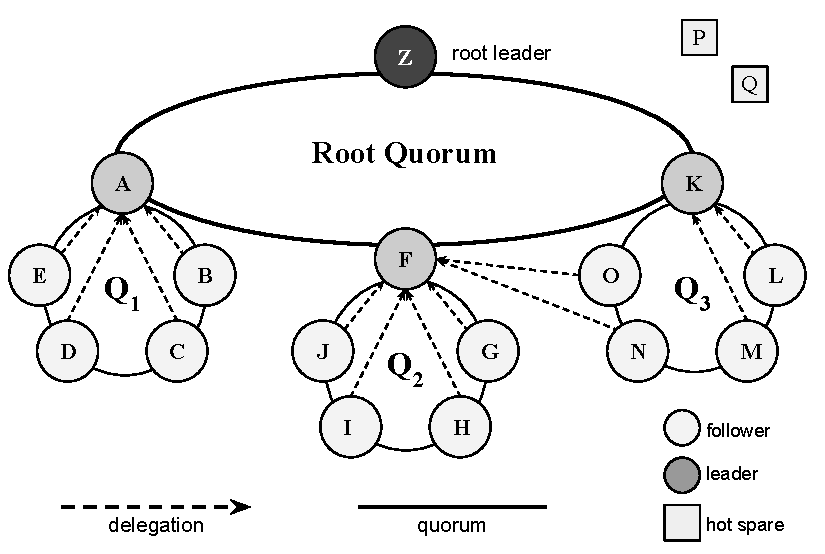
\includegraphics[width=0.5\textwidth]{figures/election3}
    \caption{All replicas are members of the \roo, but \sub peers usually delegate their votes
      to their leader. Generalized delegation allows replicas $r_N$ and $r_O$ to
      delegate votes to a different leader. Hot spares $r_P$ and $r_Q$
      are available to replace failed replicas. They participate in the \roo
      even though not assigned to a \sub.}
    \label{fig:tiers}
\end{figure}

\para{\Subs:}
The \roo partitions the namespace across multiple \subs, each with a
disjoint portion as its scope.
The intent of \sub localization is ensure that the \emph{domain} of a
client, the portion of the namespace it accesses, is entirely within the
scope of a local, or nearby, \sub.
If true across the entire system, each client interacts with only one
\sub, and \subs do not interact at all during execution of a single
epoch.
This \emph{siloing} of client accesses simplifies implementation of strong
consistency guarantees and allows better performance.


Each \sub, $q_i$, elects a leader to coordinate local decisions.
Fault tolerance of the \sub is maintained in the usual way, detecting leader
failures and electing new leaders from the peers.
\Subs do not, however, ever change system membership on their own. \Sub
membership is always defined in the \roo.

Client namespace accesses are forwarded to the leader of the \sub for the
appropriate part of the namespace.
The underlying Raft semantics ensure that leadership changes do not result in
loss of any commits.
Hence, individual- or multiple-client accesses to a single \sub are totally
ordered.
\emph{Remote accesses}, or client accesses to other than their local \sub, are
transparent to the primary protocol. However, creation of a single shared log
of all system operations requires remote accesses to be logged (Section~\ref{sec:log}).

\subsection{Delegation}
\label{sec:delegations}
Fault tolerance scales with increasing
system size.
The \roo's membership is, at least logically, the set of all system replicas,
at all times.
However, running consensus elections across large systems is inefficient in
the best of cases, and prohibitively slow in a geo-replicated environment.
\Roo decision-making is kept tractable by having replicas
\emph{delegate} their votes, usually to their leaders, for a finite duration.
With leader delegation, the root membership effectively consists of the set of
\sub leaders.
Each leader votes with a count describing its own and peer votes from its
\sub.

Consider an alternative leader-based approach where \roo membership is
defined as the current set of \sub leaders.
Both delegation and the leader approach have clear advantages in
performance and flexibility over direct votes
of the entire system.
However, the leader approach dramatically decreases fault tolerance.
Furthermore, the \roo becomes unstable in the leader approach as its
membership changes during partitions or \sub elections.
% Furthermore, \roo membership changes with \sub leaders and at \sub
% repartitions in the leader approach.
These changes would require heavyweight \emph{joint
consensus} decisions in the \roo for correctness in Raft-like protocols~\cite{raft}.

With delegation, however, \roo membership is always the entire system and remains
unchanged over \sub re-configuration.
Delegation is essentially a way to optimistically shortcut contacting every
replica for each decision.
\Sub repartitioning merely implies that a given replica's vote might need to be
delegated to a different leader.

Delegation does add one complication: the \roo leader must know all
vote delegations to request votes when committing epoch changes.
We deal with this issue, as well as the requirement for a nuclear option
(Section~\ref{sec:nuclear}), by simplifying our protocol.
Instead of sending vote requests just to \sub leaders,
 \textbf{the \roo leader sends vote requests to all system replicas.}
This is true even for \emph{hot spares}, which are not currently in any
\sub.

This is correct because vote requests now reach all replicas, and because
replicas whose votes have been delegated merely ignore the request.
We argue that it is also efficient, as a commit's efficiency depends only on
receipt of a majority of the votes.
Large consensus groups are generally slow (see Section~\ref{sec:evaluation})
not just because of communication latency, but because large groups in a
heterogeneous setting are more likely to include replicas on very slow hosts
or networks.
In the usual case for our protocol, the \roo leader still only needs to wait
for votes from the \sub leaders.
Leaders are generally those that respond more quickly to timeouts, so the
speed of \roo operations is unchanged.
% Not generally true, as timeouts are stochastic.

\subsection{Epoch Transitions}
An epoch change is initiated by the leader in response to one of several events,
including: (i) a namespace repartition request from a \sub leader, (ii) notification of join requests
by new replicas, (iii) notification of failed replicas, and (iv) changing locations or
network conditions that suggest re-assignment of replicas to existing \subs.

The root leader transitions to a new epoch through the normal commit phase in
the \roo.
The command proposed by the leader is an enumeration of the new \sub
partition, namespace partition, and assignment of namespace portions to
specific \subs.
The announcement may also include initial leaders for each \sub, with the
usual rules for leader election applying otherwise, or if the assigned leader
is unresponsive.
Upon commit, the operation serves as an \emph{announcement} to \sub leaders.
\Sub leaders repeat the announcement locally, disseminating full knowledge of
the new system configuration, and eventually transition to the new epoch by
committing an \texttt{epoch-change} operation locally.

The epoch change is lightweight for \subs that are not directly affected by
the underlying re-configuration.
If a \sub is being changed or dissolved, however, the \emph{epoch-change}
commitment becomes a tombstone written to the logs of all local replicas.
No further operations will be committed by that version of the subgroup, and
the local shared log is archived and then truncated.
Truncation is necessary to guarantee a consistent view of the log within a
\sub, as peers may have been part of different \subs, and thus have different
logs, during the last epoch.
Replicas then begin participating in their new \sub instantiation.
In the common case where a \sub's membership remains unchanged across the
transition, an \texttt{epoch-change} may still require additional mechanism
because of changes in namespace responsibility.

\para{Fuzzy Handshakes: }
Epoch handshakes are required whenever the namespace-to-\sub mapping changes across an
epoch boundary.
HC separates epoch transition announcements in the
\roo from implementation in \subs.
Epoch transitions are termed \emph{fuzzy} because
\subs need not all transition synchronously.
There are many reasons why a \sub might be slow.
Communication delays and partitions might delay notification.
Temporary failures might block local commits.
A \sub might also delay transitioning to allow a local burst of activity to
cease such as currently running transactions\footnote{The HC protocol
discussed in this paper does not currently support transactions.}.
Safety is guaranteed by tracking \sub dependencies across the epoch boundary.

\begin{figure}[t]
\centering
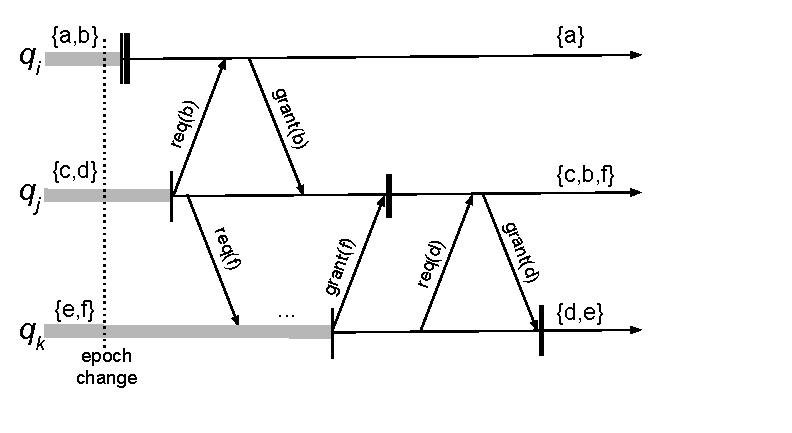
\includegraphics[width=.6\textwidth]{figures/namespaceHandoff}
\vspace{-.2in}
\caption{Readiness to transition to the new epoch is marked by a thin vertical bar; actual
  transition is the thick vertical bar.  Thick gray lines indicate
  operation in the previous epoch.  \Sub $q_j$ transitions from tag ${c,d}$ to
  ${c,b,f}$, but begins only after receiving version
  information from previous owners of those tags.  The request to $q_k$ is only answered
  once $q_k$ is ready to transition as well.}
\vspace{-.2in}
\label{fig:handoff}
\end{figure}
\para{Example:}
Figure~\ref{fig:handoff} shows an epoch transition where the scopes of
$q_i$, $q_j$, and $q_k$ change across the transition as follows:
\begin{align*}
  \label{eq:3}
  q_{i,x-1} = t_a, t_b  &\longrightarrow q_{i,x} = t_a\\
  q_{j,x-1} = t_c, t_d  &\longrightarrow q_{j,x} = t_c,t_d,t_f\\
  q_{k,x-1} = t_e, t_f  &\longrightarrow q_{k,x} = t_d,t_e
\end{align*}
All three \subs learn of the epoch change at the same time, but become ready
with varying delays.
These delays could be because of network lags or ongoing local activity.
\Sub $q_i$ gains no new tags across the transition and moves immediately to the new epoch.
\Sub $q_j$'s readiness is slower, but then it sends requests to the
owners of both the new tags it acquires in the new epoch.
Though $q_i$ responds immediately, $q_k$ delays its response until locally
operations conclude.
Once both handshakes are received, $q_j$ moves into the new epoch, and $q_k$
later follows suit.

These bilateral handshakes allow an epoch change to be implemented
incrementally, eliminating the need for lockstep synchronization across the entire
system.
This flexibility is key to coping with partitions and varying connectivity in
the wide area.
However, this piecewise transition, in combination with \sub re-definition and
configuration at epoch changes, also means that individual replicas \emph{may
be part of multiple \subs at a time}.

This overlap is possible because replicas may be mapped to distinct subgroups
from one epoch to the next.
Consider $q_k$ in Figure~\ref{fig:handoff} again.
Assume the epochs shown are $e_x$ and $e_{x+1}$.
A single replica, $r_a$, may be remapped from \sub $q_{k,x}$ to \sub $q_{i,x+1}$ across the
transition.
\Sub $q_{k,x}$ is late to transition, but $q_{i,x+1}$ begins the new epoch
almost immediately.
Requiring $r_a$ to participate in a single \sub at a time would potentially delay
$q_{i,x+1}$'s transition and impose artificial synchronicity constraints on the
system.
One of the many changes we made in the base Raft protocol is to
allow a replica to have multiple distinct shared
logs.
Smaller changes concern the mapping of requests and responses to the appropriate
consensus group.


\subsection{Fault Tolerance}

We assert that consensus at the leaf replicas is correct and safe because decisions are
implemented using well-known leader-oriented consensus approaches.
Hierarchical consensus therefore has to demonstrate linearizable correctness and safety
between \subs for a single epoch and between epochs.
Briefly, linearizability requires external observers to view operations to objects as
instantaneous events.
Within an epoch, subquorum leaders serially order local accesses, thereby guaranteeing
linearizability for all replicas in that quorum.
% Remote accesses and the internal invariant also enforce linearizability of accesses
% between \subs.

Epoch transitions raise the possibility of portions of the namespace being re-assigned from one \sub to
another, with each \sub making the transition independently.
Correctness is guaranteed by an invariant requiring \subs to delay serving newly
acquired portions of the namespace until after completing all appropriate handshakes.


\begin{table*}[t]
  \centering
  \begin{tabular}{l|l} \hline
    \mcn{Failure Type} & \mcn{Response} \\ \hline
    \sub peer & request replica repartition from \roo \\
    \sub leader & local election, request replacement from \roo \\
    root leader & root election (with delegations)\\
    majority of majority of \subs & (nuclear option) root election after delegations
                                    timed out \\
  \end{tabular}
  \caption{Failure categories: Peer failure is detected by missed heartbeat
    messages. The rest are triggered by the appropriate election timeout.}
  \label{tab:categories}
\end{table*}

\subsubsection{Failures}
\label{sec:fault-tolerance}

During failure-free execution, the \roo partitions the system into
disjoint \subs, assigns \emph{\sub leaders}, and assigns partitions
of the tagspace to \subs.
Each \sub coordinates and responds to accesses for objects in its assigned
tagspace.
We define the system's \emph{safety} property as guaranteeing that
non-linearizable (or non-sequentially-consistent, see Section~\ref{sec:log})
event orderings can never be observed.
We define the system's \emph{progress} property as the system having enough
live replicas to commit votes or operations in the \roo.

The system can suffer several types of failures, as shown in
Table~\ref{tab:categories}.
Failures of \sub and \roo leaders are handled through the normal consensus
mechanisms.
Failures of \sub peers are handled by the local leader petitioning the \roo to
re-configure the \sub in the next epoch.
Failure of a \roo peer is the failure of \sub leader, which is handled as
above.
\Roo heartbeats help inform other replicas of leadership changes, potentially
necessary when individual \subs break down.

HC's structure means that some faults are more important than others.
Proper operation of the \roo requires the majority of replicas in the majority of \subs to
be non-faulty.
Given a system with $2m+1$ \subs, each of $2n+1$ replicas, the entire
system's progress can be halted with as few as $(m+1)(n+1)$ well-chosen
failures.
Therefore, in worst case, the system can only tolerate:
\begin{align*}
f_{worst}=mn+m+n
\end{align*}
failures and still make progress.
At maximum, HC's basic protocol can tolerate up to:
% f_{max} = (m+1)*n + m*(2n+1) = mn + n + 2mn+m = 3mn+m+n
\begin{align*}
f_{best} = (m+1)*n + m*(2n+1) = 3mn+m+n
\end{align*}
failures.
As an example, a 25/5 system can tolerate at least 8 and
up to 16 failures out of 25 total replicas.
A 21/3 system can tolerate at least 7, and a maximum of 12,
failures out of 21 total replicas.
Individual \subs might
still be able to perform local operations despite an impasse at the global level.

Total \sub failure can temporarily cause a portion of the namespace to be unserved. However, the \roo
eventually times out and moves into a new epoch with that portion assigned to another
\sub.

\subsubsection{The Nuclear Option}
\label{sec:nuclear}
Singleton consensus protocols, including Raft, can tolerate just under half of the entire system
failing.
As described above, HC's structure makes it more vulnerable to clustered failures.
Therefore we define a \emph{nuclear option}, which uses direct consensus
decision among all system replicas to tolerate any $f$ replicas
failing out of $2f+1$ total replicas in the system.

A nuclear vote is triggered by the failure of a root leader election.
A \emph{nuclear candidate}
increment's its term for the \roo and broadcasts a request for votes to all
system replicas.
The key difficulty is in preventing delegated votes and
nuclear votes from reaching conflicting decisions.
Such situations might occur when temporarily unavailable \sub leaders regain connectivity
and allow a wedged \roo to unblock.
Meanwhile, a nuclear vote might be concurrently underway.

Replica delegations are defined as intervals over specific slots.
Using local \sub slots would fall prey to the above problem, so we define
delegations as a small number (often one) of root slots, which usually
correspond to distinct epochs.
During failure-free operation, peers delegate to their leaders and are all
represented in the next root election or commit.
Peers then renew their delegations to their leaders by appending them to the
next local commit reply.
This approach works for replicas that change \subs over an epoch
boundary, and even allows peers to delegate their votes to arbitrary other
peers in the system (see replicas $r_N$ and $r_O$ in Figure~\ref{fig:tiers}).

This approach is simple and correct, but deals poorly with leader turnovers in
the \subs.
Consider a \sub where all peers have delegated votes to their leader
for the next root slot.
If that leader fails, none of the peers will be represented.
We finesse this issue by re-defining such delegations to count
root elections, root commits, \emph{and} root heartbeats.
The latter means that local peers will regain their votes for the next \roo
action if it happens after to the next heartbeat.

\para{Example:} Consider the worst-case failure situation discussed in Section~\ref{sec:fault-tolerance}: a
majority of the majority of \subs have failed.
None of the failed \sub leaders can be replaced, as none of those \subs have
enough local peers.

The first response is initiated when a replica holding delegations (or its own
vote) times out waiting for the root heartbeat.
That replica increments its own root term, adopts the prior system
configuration as its own, and becomes a root candidate.
This candidacy fails, as a majority of \sub leaders, with all of their
delegated votes, are gone.
Progress is not made until delegations time out.
In our default case where a delegation is for a single root event, this
happens after the first root election failure.

At the next timeout, any replica might become a candidate because delegations have
lapsed (under our default assumptions above).
Such a \emph{nuclear} candidate increments its root term and
sends candidate requests to all system replicas,
succeeding if it gathers a majority across all live replicas.

The first candidacy assumed the prior system configuration in its candidacy
announcement.
This configuration is no longer appropriate unless some of the ``failed''
replicas quickly regain connectivity.
Before the replica announces its candidacy for a second time, however, many of
the replica replies have timed out.
The candidate alters its second proposed configuration by recasting all such
replicas as hot spares and potentially reducing the number and size of the
subgroups.
Subsequent epoch changes might re-integrate the new hot spares if the replicas
regain connectivity.

\begin{figure}[t]
  \centering
  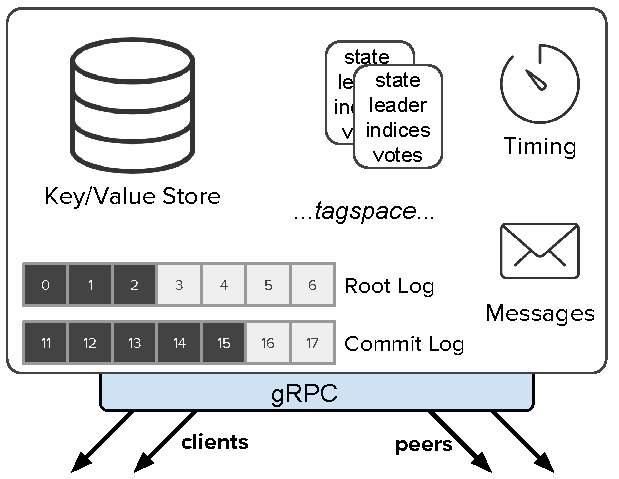
\includegraphics[width=.45\textwidth]{figures/replica.pdf}
  \caption{\sys replica. State includes both \roo and \sub}
  \label{fig:replica}
\end{figure}

\section{The Alia Key-Value Store}
\label{sec:key-store}

\sys is a linearizable key-value store implemented using Hierarchical
Consensus.
Replica structure is shown in Figure~\ref{fig:replica}.
\sys maps onto HC by using the namespace to represent the object space, and
\sub operations to commit object writes.
Reads are not committed by default, but are always served by the leader of the
appropriate \sub.
Namespace assignments in HC result in the object space being partitioned (or
sharded) across distinct \subs.

The mapping of the shared object namespace to individual \subs is the
\emph{tagset}, or the tagset partition.
An individual \emph{tag} defines a disjoint subset of the object space.
\Sub membership, \sub leaders, and tagsets are all proposed and committed in
epoch changes in the \roo.

As \sys commits writes through HC, the shared logs provide a complete version
history of all distributed objects.
\Sub leaders use in-core caches to provide fast access to recently accessed
objects in the local \sub's tag.
Replicas perform background anti-entropy~\cite{dynamo,bayou,bayou2}, disseminating
log updates a
user-defined number of times across the system.

The most complex portion of the \sys protocol is in handling data-related
issues at epoch transitions.
Transitions may cause tags to be transferred from one \sub to another, forcing
the new leader to load state remotely to serve object
requests.
Transitions handshakes are augmented in three ways.
First, an \sys replica can demand-fetch an object version from any other
system replica.
Second, epoch handoffs contain enumerations of all current object versions,
though not the data itself.
Knowing an object's current version gives the new handler of a tag the ability
to demand fetch an object that is not yet present locally.
Finally, handshakes start immediate fetches of the in-core version cache from
the leader of the tag's \sub in the old epoch to the leader in the new.

We do not currently gather the entire shared log onto a single replica because
of capacity and flexibility issues.
Capacity is limited because our system and applications are expected to be
long-lived.
Flexibility is a problem because HC, and applications built on HC, gain much
of their value from the ability to pivot quickly, whether to deal with changes in the
environment or for changing application access patterns.
We require handoffs to be as lightweight as possible to preserve this
advantage.

Pushing all writes through \sub commits and serving reads at leaders allows us
to guarantee that accesses are linearizable (Lin), which is the
strongest non-transactional
consistency~\cite{linearizability,attiya_sequential_1994}.
As a recap, linearizability is a combination of atomicity and timeliness
guarantees about accesses to a single object.
Both \texttt{reads} and \texttt{writes} must appear atomic, and also instantaneous at some time between
a request and the corresponding response to a client.
\texttt{Reads} must always return the latest value.
This implies that reads return values are consistent \emph{with any observed
ordering}, i.e., the ordering is \emph{externalizable}~\cite{externalizable}.

Linearizability of object accesses can be \emph{composed}.
If operations on each object are linearizable, the entire object space is also
linearizable.
This allows our \subs to operate independently while providing a globally
consistent abstraction.

\begin{figure*}[t]
\centering
\subfigure[Default ordering: $w_{i,1}\rightarrow w_{i,3}\rightarrow w_{j,1}\rightarrow w_{j,3}$] {
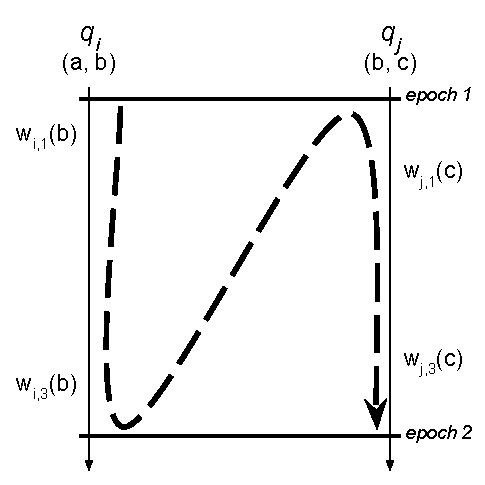
\includegraphics[width=.35\textwidth]{figures/eventOrdering}
\label{fig:eventOrdering}
}
\hspace{.65in}
\subfigure[Remote writes add additional ordering constraints: $w_{i,1}
\rightarrow w_{i,2}\rightarrow w_{j,3}$, and $ w_{j,1} \rightarrow w_{j,2} \rightarrow w_{i,3}$] {
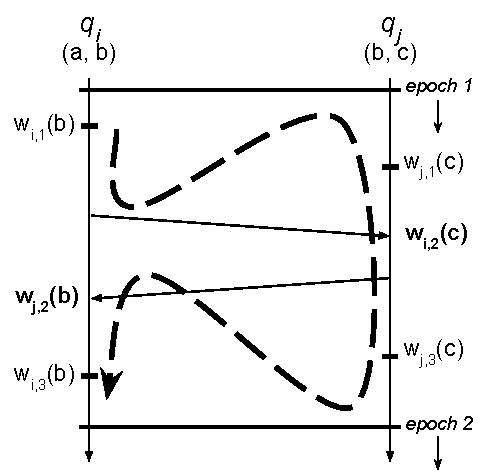
\includegraphics[width=.35\textwidth]{figures/eventOrdering3}
\label{fig:eventOrderingRemote}
}
\caption{Dotted lines show one possible event ordering for replicas $G_1$ (responsible for
  objects $a$ and $b$), and $G_2$ ($c$ and $d$). Each remote write establishes a partial
  ordering between events of the sender before the sending of the write, and the writes by the receiver
  after the write is received.}
\label{fig:events}
\end{figure*}

\section{Globally Consistent Logs}
\label{sec:log} Our default use case is in providing linearizable access to an
object store.
Though this approach allows us to guarantee all observers will see
linearizable results of object accesses in real-time, the system is not able to enumerate a
total order, or create a linearizable shared log.
Such a linear order would require fine-grained (expensive) coordination across
the entire system, or fine-grained clock synchronization~\cite{spanner}.
Though many or most distributed applications (objects stores, file systems,
etc.)
will work directly with HC, shared logs are a useful building block for
distributed systems.

HC \emph{can} be used to build a sequentially consistent (SC) shared log.
Like Lin, SC requires all observers to see a single total ordering.
SC differs in that this total ordering does not have to be externalizable.
Instead, it merely has to conform to local operation orders and all reads-from
dependencies.

Figure~\ref{fig:eventOrdering} shows a system with \subs $q_i$ and $q_j$, each of which
performs a pair of writes.
Without cross-\sub reads or writes, ordering either
\sub's operations first creates a SC total ordering: $q_i \rightarrow q_j$ (``happened-before''~\cite{lamport_time_1978})
implies $w_{i,1} \rightarrow w_{i,3} \rightarrow w_{j,1} \rightarrow w_{j,3}$,
for example.

By contrast, the \subs in Figure~\ref{fig:eventOrderingRemote} create
additional dependencies by issuing remote writes to other \subs: $w_{i,2}
\rightarrow w_{j,3}$ and $w_{j,2} \rightarrow w_{i,3}$.
Similar dependencies result from remote reads.

These dependencies cause the epochs to be split (not shown in picture).
The receipt of write $w_{i,2}$ in $q_j$ causes $q_{j,1}$ to be split into
$q_{j,1.1}$ and $q_{j,1.2}$.
Likewise, the receipt of write $w_{j,2}$ into $q_i$ causes $q_i$ to be split
into $q_{i,1.1}$ and $q_{i,1.2}$.
Any topological sort of the subepochs that respects these orderings, such as
$q_{i,1.1} \rightarrow q_{j,1.1} \rightarrow q_{j,1.2} \rightarrow q_{i,1.2}$,
results in a valid SC ordering.

Presenting a sequentially consistent global log across the entire system,
then, only requires tracking these inter-\sub data accesses, and then
performing an $\mathcal{O}(n)$ merge of the subepochs.

\para{Versus linearizability:} By definition, this log's ordering respects any
externally visible ordering of cross-\sub accesses (accesses visible to the
system).
However, the log does not necessarily order other accesses according to
external visibility.
The resulting shared log could not be mined to find causal relationships
between accesses through external communication paths unknown to the system.

For example, assume that log events are published posts, and that one user claimed
plagiarism.
The accused would not be able to prove that his post came first unless there
were some causal chain of posts and references visible to the protocol.

\section{Implementation}
\label{sec:implementation}

\sys implements a replicated key-value store with strong consistency via the
Hierarchical Consensus protocol.
An \sys cluster is composed of $N$ replica processes that each manage a
partial replica of the object space.
Hierarchical Consensus with modified Raft as the underlying consensus
protocol exports a linearizable order of accesses to the distributed key-value
store.
\sys and the HC library are implemented in Golang use gRPC~\cite{grpc} for
communication.
The system is implemented in 7,924 lines of code, not including standard
libraries or support packages.

Each \sys replica~(Figure \ref{fig:replica}) implements an event loop that responds to timing events,
client requests, and messages from peers.
Events may cause the replica to change state, modify a command log, broadcast
messages to peers, modify the key-value store, or respond to a client.
% Events must be handled one at a time in the order they arrive at the replica
% to ensure correct behavior.
Event
handlers need to aggressively lock shared state for correctness because Golang and
gRPC make extensive use of multi-threading.
% This conflicts with the need to avoid complete serialization by exploiting concurrency.
The balance between correctness and concurrency-driven performance leads to
increasing complexity and tighter coupling between components, one that
foreshadows extra-process consistency concerns that have been noted in other
work~\cite{chandra_paxos_2007,raft}.

\para{Consistency:} \sys guarantees completely linearizable data accesses
to individual objects.
An object \texttt{write} must be committed to the \sub log before it can be
applied to the key-value store.
Any \texttt{write} that is not successfully committed is dropped without being
applied to the store, requiring clients to retry the \texttt{write}.
Object \texttt{reads} are serialized with respect to all \texttt{writes} by
ensuring they are satisfied by the leader.
Non-leader replicas redirect clients to the appropriate leader for the
requested object.
\sys also supports a more relaxed model where \texttt{reads} can be satisfied
by any replica in the \sub from values in the shared log~\cite{calvin}.
Shared logs on peer replicas are not guaranteed to be up-to-date, though the degree
of staleness can be parameterized.

\para{Timing:} The computing and network environment of a distributed system
plays a large role in determining not just the performance of the system, but
also its behavior.
A simple example is the election timeout parameter of the Raft consensus
protocol, which must be much greater than the average time to
broadcast and receive responses, and much less than the mean time
between failures~\cite{raft,etcd}.
If this requirement is not met,
leader may be displaced before heartbeat messages arrive, or the system will be
unable to recover when a leader fails.
As a result, the relationship between timeouts is critically dependent on the mean
latency ($\lambda_{\mu}$) of the network.
Howard~\cite{raftRefloated} proposes  $T = \lambda_{\mu} +
2\lambda_{\sigma}$ to determine timeouts based on the distribution of observed
latencies, sets the heartbeat as $\frac {T} {2}$, and the election timeout as
the interval $U(T,2T)$.
We parameterize our timeouts (Table~\ref{tab:ticks}) on
latency measurements made before we ran our experiments.
Monitoring and adapting to network conditions is part of ongoing work.

\begin{table}[t]
  \centering
  \begin{tabular}{l|l|l} \hline
\mcn{Name} & \mcn{Time} & \mcn{Actions} \\ \hline
sub heartbeat& 1T & sub leader heartbeat\\
sub leader & 2-4T & new sub election\\ \hline
root heartbeat & 10T & root leader heartbeat \\
root election & 20-40T & new root election \\ \hline
\lb{obligation} & \lb{50T} & \roo may re- \\
 &  & allocate the tag
  \end{tabular}
  \caption{Parameterized timeouts in our implementation. The \emph{obligation} timeout
    stops a partitioned \sub after an extended time without contact to the
    rest of the system. $T=10 \mbox{ msec}$ for our experiments on Amazon EC2.}
  \label{tab:ticks}
\end{table}

\para{Protocol:} An \sys replica implements multiple instantiations of the
Raft protocol, which we have modified in several ways.
% Raft proposes two phases: an election phase implemented by the
% \texttt{RequestVote} RPC and an append entries phase implemented by the
% \texttt{AppendEntries} RPC.
% \sys consensus instantiations also have two phases, leader election and log
% modification, but differ in purpose and integration with other instantiations.
%
Every replica must run one instantiation of the \textit{root consensus
protocol}.
Replicas may also run one or more instantiations of the \textit{commit
consensus protocol} if they are assigned to a \sub.
% The root consensus protocol implements the two phases with the
% \texttt{DelegatedVote} and \texttt{Repartition} RPCs.
Vote delegation is the subject of Section~\ref{sec:delegations}.
Repartition decisions move the system between
epochs with a new configuration and tagspace, and can only be initiated by
messages from peers or monitoring processes.
A successful repartition results in a new epoch, tagspace, and \sub topology
committed to the root log.
\texttt{Repartition} messages also serve to notify the network about events
that do not require an epoch change, such as the election of a new \sub leader
or bringing a failed node back online.
% The \textit{commit consensus protocol} implements \texttt{Vote} and
% \texttt{CommitValue} RPCs similar to the original Raft protocol.

\para{Changes to base Raft:} In addition to major changes, such allowing
replicas to be part of multiple quorums simultaneously, we also made many
smaller changes that had pervasive effects.
One change was including the \textit{epoch} number alongside the term in all
log entries.
The epoch is evaluated for invariants such as whether or not a replica can
append an entry or if a log is as up to date as a remote log.

Vote delegation requires changes to vote counting.
Since our \roo membership actually consists of the entire system, all replicas
are messaged during root events.
All replicas reply, though most with a ``zero votes'' acknowledgment.
The root uses observed vote distributions to inform the ordering of future
consensus messages (sending requests first to replicas with votes to cast),
and uses timeouts to move non-responsive replicas into ``hot spares'' status.

We allow \texttt{AppendEntries} requests in \subs to aggregate multiple client
requests into a single consensus round.
Such requests are collected while an outstanding commit round is ongoing, then
sent together when that round completes.
The \roo also aggregates all requests within a minimum interval into a single
new epoch-change/reconfiguration operation to minimize disruption.

Commits are observed by the leader once a majority of replicas respond
positively.
Other replicas learn about the commit only on the next message or heartbeat.
Root epoch changes and heartbeats are designed to be rare, meaning that epoch
change commits are not seen promptly.
We modified the root protocol to inform \subs of the change by sending an
additional heartbeat immediately after it observes a commit.

Replicas may be part of both a \sub and the \roo, and across epoch boundaries
may be part of multiple \subs.
In principle, a high performance replica may participate in any number of
\subs.
We therefore allow replicas to accommodate multiple distinct logs with
different access characteristics.

Peers that are either slow or with unsteady connectivity are occasionally left
behind at \sub leader or epoch changes.
Root heartbeats containing the current system configuration are broadcast to
all replicas and serve to bring them up to date.

Finally, consensus protocols often synchronously write state to disk before
responding to remote requests.
This allows replicas that merely crash to reboot and rejoin the ongoing
computation after recovering state from disk.
Otherwise, these replicas need to go through heavyweight leave-and-rejoin
handshakes.
Our system avoids these synchronous writes by allowing epochs to re-join a
\sub at the next epoch change without any saved state, avoiding these
handshakes altogether.


\hmm{
- anti-entropy  (two ints)
  - will be merkle trees
  - key-value store level
  - why
    - all doing is speeding up handoff
    - durability
- separate logs
- root leader doesn't change unless he dies, survives effect root quorum
changes.

\begin{equation}
tick = 2 * \lambda_\mu + 4 * \lambda_\sigma
\end{equation}
- delegations survive sub changes

- mark on ack does delegate

- hot spares are part of the vote  100\%  replicas participate

- so by sending to all
  - we are only listening to 3, rather than more w/ possibility of being
  slowed by slowest members
  - fastest responders will be elected leaders in subs (ben says natural)
  - but we nominate (as optimization)
    - root keeps track of who responds first

root
- two separate commands
}



\hmm{We note that the safety violations Ongaro et al.~\cite{raft} use to
motivate joint consensus apply only when more than one node is added
at a time, and not at all when nodes are removed.

For the former, assume a system with $2m+1$ nodes. Assume a decision to
increase the size by two nodes is taken and acknowledged by a total of
$m+1$ nodes, followed by the failure of all of those acknowledgers.
The remaining $m$ nodes, together with the two new nodes, can constitute.
}

\begin{figure*}[!t]
  \centering
  \subfigure[Mean throughput of workloads of up to 120 clients.] {
    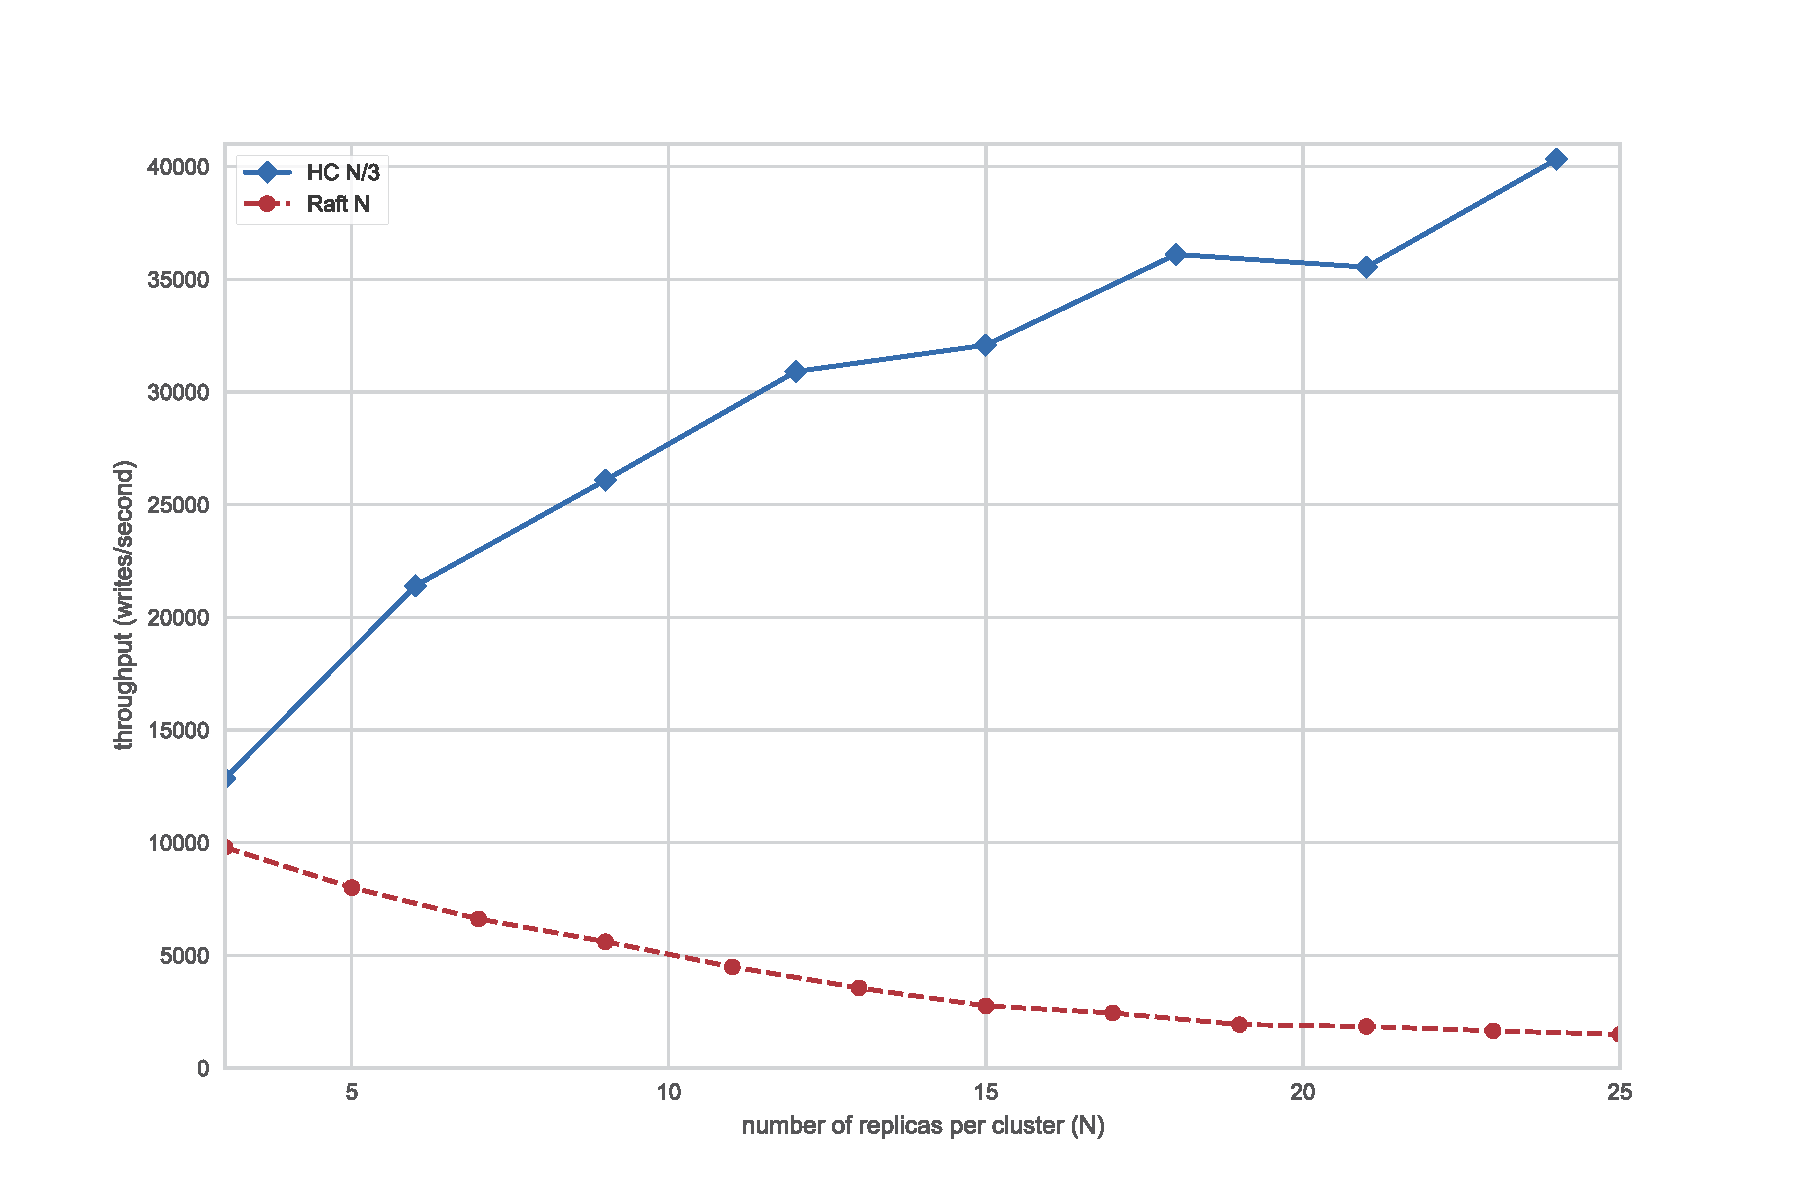
\includegraphics[width=.48\textwidth]{figures/scaling}
    \label{fig:raftMaxThroughput}
  }
  \subfigure[Throughput vs workload for different HC cluster sizes.] {
    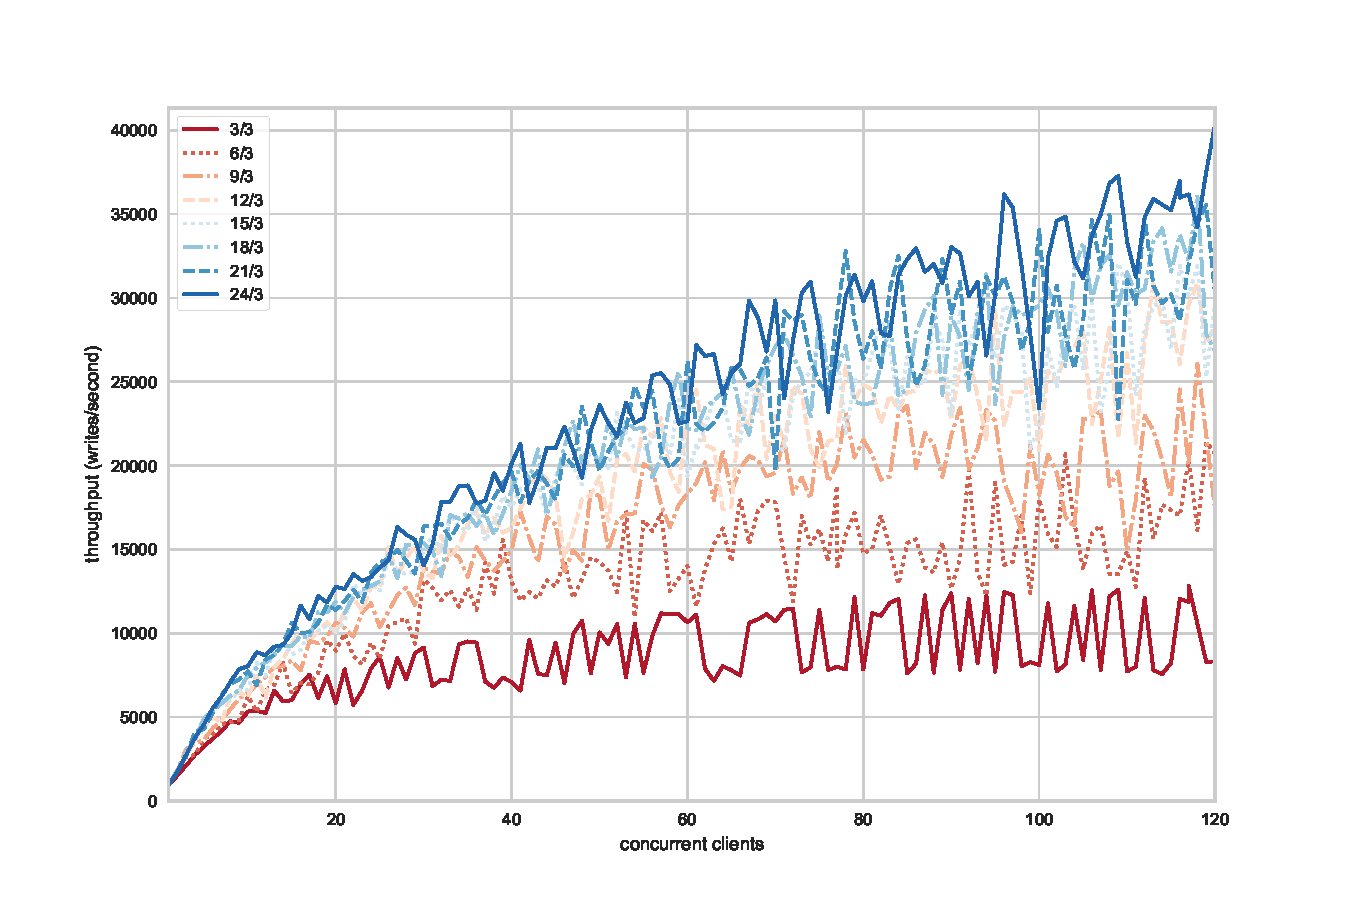
\includegraphics[width=.48\textwidth]{figures/hc_throughput_workload}
    \label{fig:hcThroughput}
  }
  \caption{Performance of distributed consensus with an increasing workload of concurrent clients. Performance is measured by throughput, the number of writes committed per second.}
  \label{fig:scaling}
\end{figure*}

\section{Evaluation}
\label{sec:evaluation}


\sys was designed to adapt both to dynamic workloads as well as
variable network conditions.
We therefore evaluate \sys in two distinct environments: a homogeneous data
center and a heterogeneous real-world network.
The homogeneous cluster is hosted on Amazon EC2 and includes 26
``t2.medium'' instances: dual-core virtual machines running in a single VPC
with inter-machine latencies of $\lambda_{\mu}=0.399ms$ and
$\lambda_{\sigma}=0.216ms$.
These machines are cost effective and, though lightweight, are easy to scale
to large cluster sizes as workload increases.
Experiments are set up such that each instance runs a single replica process
and multiple client processes.

The heterogeneous cluster (UMD) consists of several local machines distributed
across a wide area, with inter-machine latencies ranging from
$\lambda_{\mu}=2.527ms$,
$\lambda_{\sigma}=1.147ms$ to $\lambda_{\mu}=34.651ms$,
$\lambda_{\sigma}=37.915ms$.
Machines in this network are a variety of dual and quad core desktop servers
that are solely dedicated to running these benchmarks.
Experiments on these machines are set up so that each instance runs multiple
replica and client processes co-located on the same host.
In this environment, localization is critical both for performance but also
to ensure that the protocol can elect and maintain consensus leadership.
The variability of this network also poses challenges that \sys is uniquely
suited to handle via \roo-guided adaptation.
We explore two distinct scenarios in Figure~\ref{fig:series} using
this cluster; all other experiments were run on the EC2 cluster.

\para{Scaling:} \sys is partially motivated by the need to scale strong
consistency to large cluster sizes.
We based our work on the assumption that consensus performance decreases as
the quorum size increases, which we confirm empirically in
Figure~\ref{fig:raftMaxThroughput}.
This figure shows the maximum throughput against system size for a
variety of workloads, up to 120 concurrent clients.
A workload consists of one or more clients continuously sending writes of a
specific object or objects to the cluster without pause.
% More clients means more concurrent writes to the system and therefore the
% potential for consistency failures.

Standard consensus algorithms, Raft in particular, scale poorly with
uniformly decreasing throughput as nodes are added to the cluster.
Commit latency increases with quorum size as the system has
to wait for more responses from peers, thereby decreasing overall throughput.
Figure~\ref{fig:scaling} clearly shows the multiplicative advantage of \sys's
hierarchical structure, though \sys does not scale linearly as we had
expected.

There are at least two factors currently limiting the HC throughput shown
here.
First, the HC \subs for the larger system sizes are not saturated.
A single 3-node \sub saturates at around 25 clients and this experiment has
only about 15 clients per \sub for the largest cluster size.
We ran experiments with 600 clients, saturating all \subs even in the 24-node
case.
This throughput peaked at slightly over 50,000 committed writes per second,
better but still lower than the linear scaling we had expected.

We think the reason for this ceiling is hinted at by
Figure~\ref{fig:hcThroughput}.
This figure shows increasingly larger variability with increasing system
sizes.
A more thorough examination of the data shows widely varying performance
across individual \subs in the larger configurations.
We suspect that the cause is either VM misconfiguration or misbehavior.
We are adding more instrumentation to diagnose the problem.

\begin{figure}[t]
  \centering
  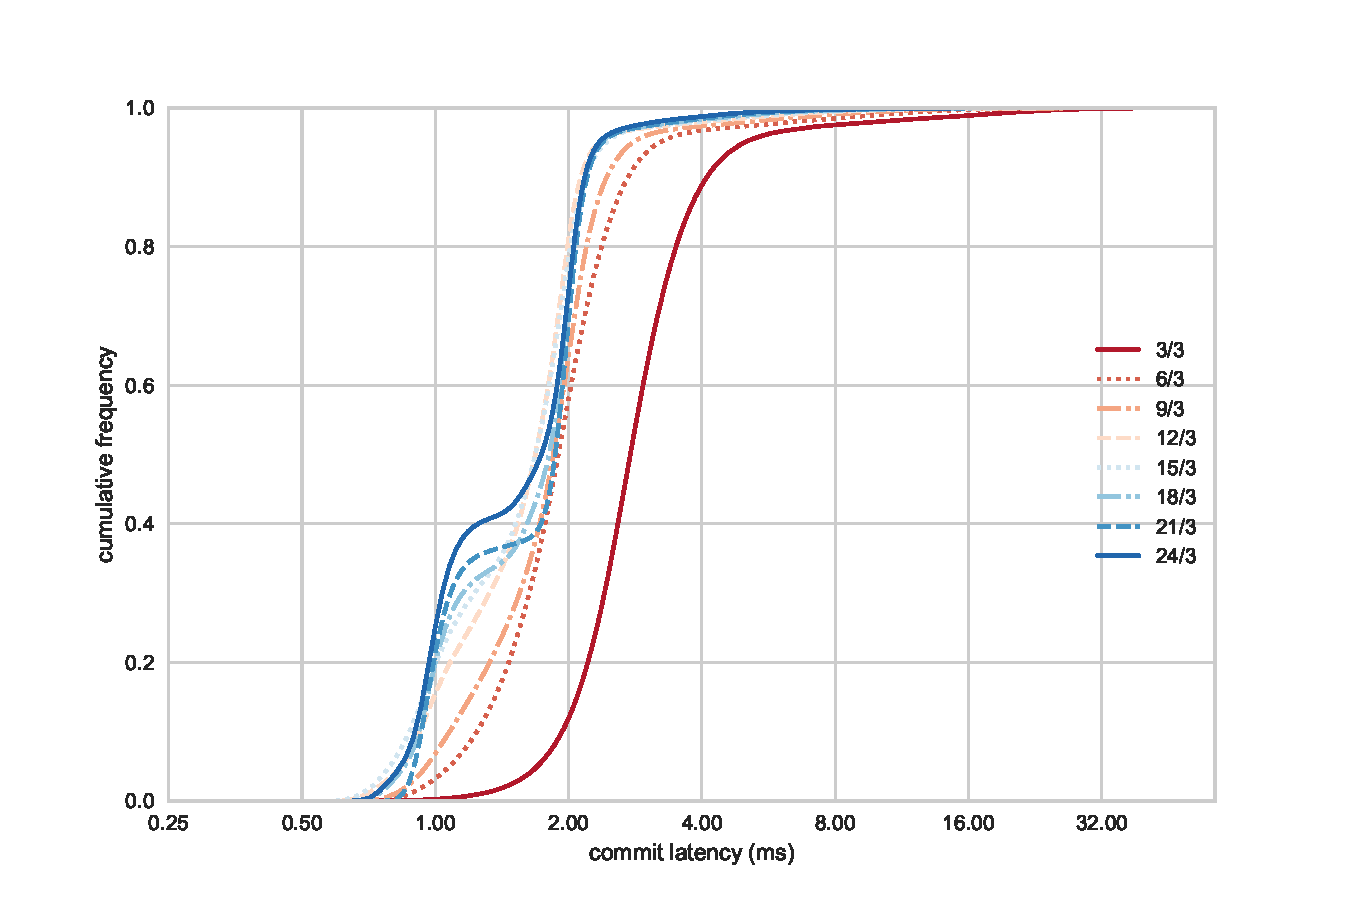
\includegraphics[width=.48\textwidth]{figures/ec2_latency_cumfreq.pdf}
  \caption{Client-observed cumulative latency distributions with 25 clients versus system size.}
  \label{fig:latency}
\end{figure}

The effect of saturation is also demonstrated in Figure~\ref{fig:latency},
which shows cumulative latency distributions for different
system sizes holding the  workload (number of concurrent clients) constant.
The fastest (24/3) shows nearly 80\% of client write requests
being serviced in under 2 msec.
Larger system sizes are faster because the smaller systems suffer from
contention (25 clients can saturate a single \sub).
Because throughput is directly related to commit latency, throughput
variability can be mitigated by adding additional subquorums to balance
load.
% The hump in the middle for larger system sizes appears to be from clients ending up
% co-located with servers.

\begin{figure*}[t]
  \centering
  \subfigure[9/3 system adapting to changing client access patterns by repartitioning the
  tag space so that clients are co-located with \subs that serve tags they need.] {
    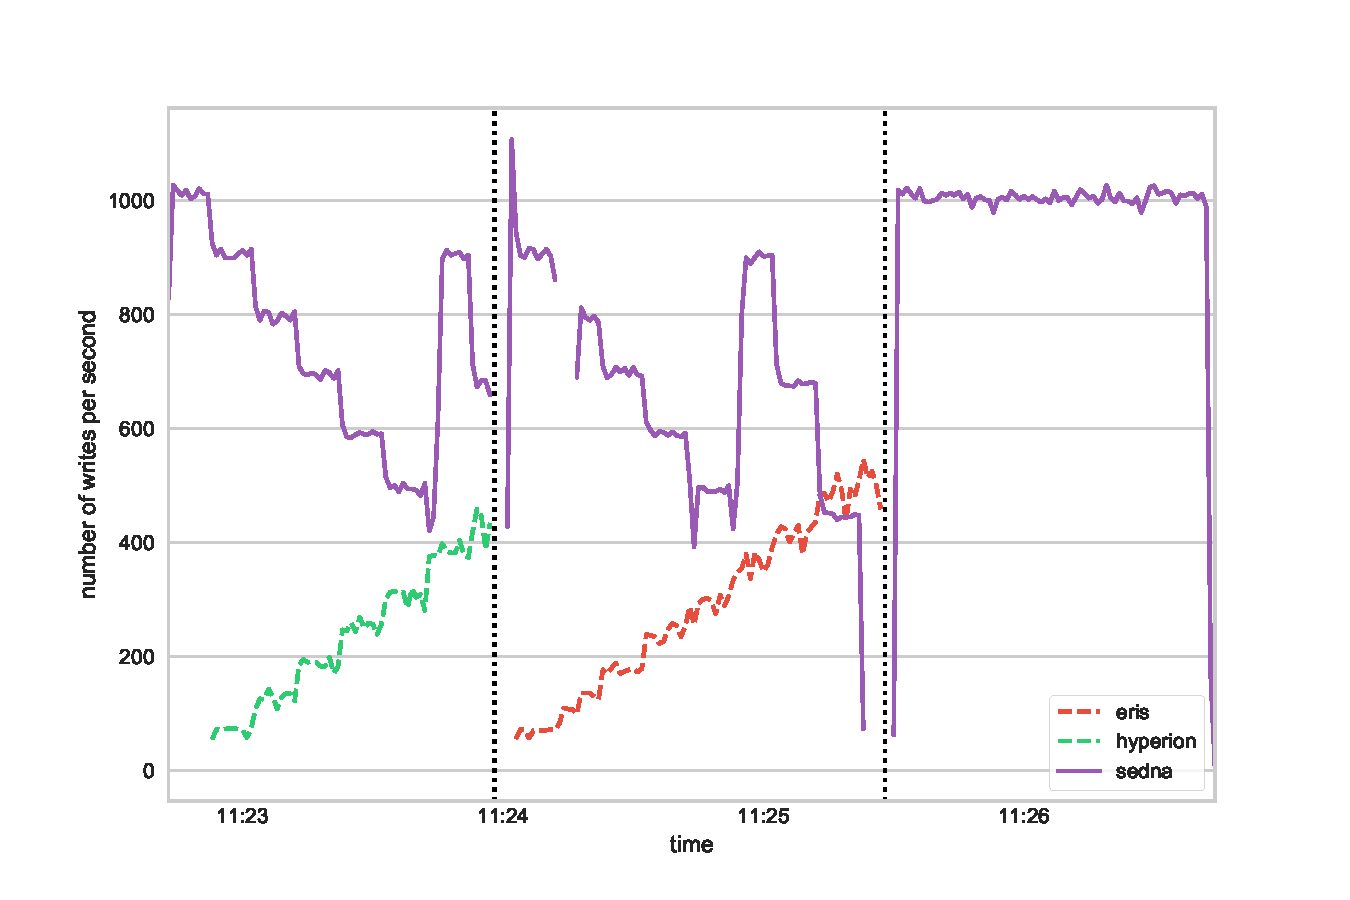
\includegraphics[width=.48\textwidth]{figures/umd_sawtooth}
    \label{fig:sawtooth}
  }
  \subfigure[9/3 System that adapts to failure (partition) of entire \sub. After timeout,
  the \roo re-partitions the tag allocated to the failed \sub among the other two \subs.] {
    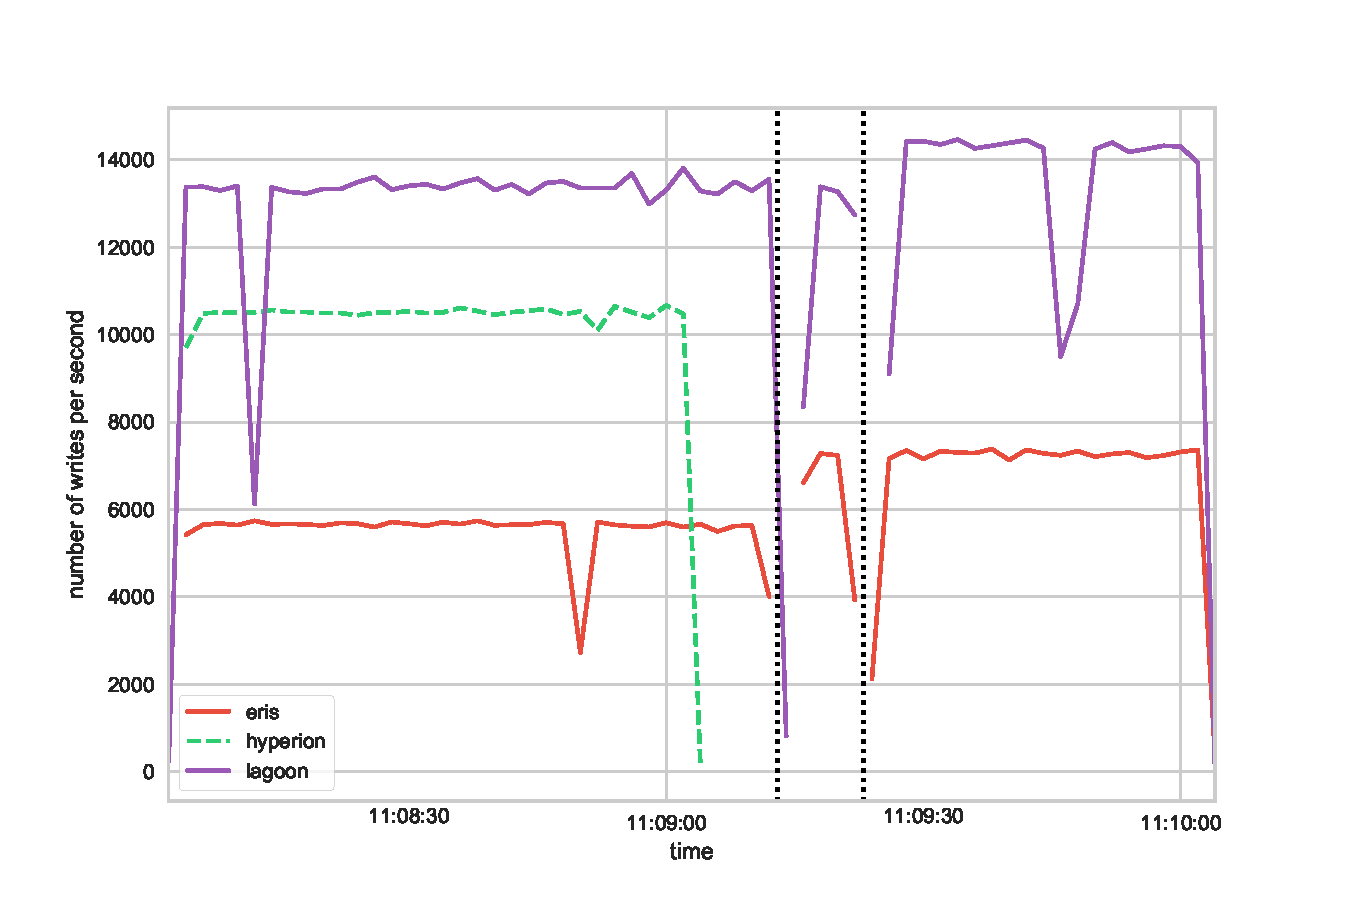
\includegraphics[width=.48\textwidth]{figures/umd_fault_tolerance}
    \label{fig:fault}
  }
  \caption{Both experiments with systems of 9 replicas arranged into 3 \subs.}
  \label{fig:series}
\end{figure*}

\para{Adaptivity:} Besides pure performance and scaling, \sys is also
motivated by the need to adapt to varying environmental
conditions.
In the next set of experiments, we explore two common runtime scenarios that
motivate adaptation:
shifting client workloads and failures.
We show that \sys is able to adapt and recover with little loss in
performance. These scenarios are shown in Figure~\ref{fig:series} as
throughput over time, where vertical dotted lines indicate an epoch change.

The first scenario, described by the time series in Figure~\ref{fig:sawtooth}
shows an \sys 3-replica configuration moving through two epoch changes.
Each epoch change is triggered by the need to localize tags accessed by
clients to nearby \subs.
% The experiment was run over machines with widely varying latency.
The scenario shown starts with all clients co-located with the \sub serving
the tag they are accessing.
However, clients incrementally change their access patterns first to a tag
located on one remote \sub, and then to the tag owned by the other.
In both cases, the \roo adapts the system by repartitioning the tagspace such
that the tag defining their current focus is served by the co-located \sub.

Finally, Figure~\ref{fig:fault} shows a 3-\sub configuration where one entire
\sub becomes partitioned from the others.
After a timeout, the root uses an epoch change to re-allocate the tag of the
partitioned \sub over the two remaining \subs.
The partitioned \sub eventually has an \emph{obligation timeout}, after which
the \roo is not obliged to leave the tag with the current \sub.
The tag may then be re-assigned to any other \sub.
Timeouts are structured such that by the time an obligation timeout fires,
the \roo has already re-mapped that \sub's tag to other \subs.
As a result, the system is able to recover from the partition as fast as
possible.
Note that in this figure, the repartition occurs through two epoch changes,
the first allocating part of the tagspace to the first \sub, and the
second allocating the rest of the tag to the other.
Gaps in the graph are periods where the \subs are electing local leaders.
This may be optimized by having leadership assigned or maintained through
root consensus.
% None of the \subs is pegged, which is why the throughput goes up.


\section{Related Work}
\label{sec:related}

Our principle contribution is Hierarchical Consensus, a general technique to
compose consensus groups, maintain consistency invariants over large
systems, and adapt to changing conditions and application loads.
HC is related to the large body of work improving
throughput in distributed consensus over the Paxos
protocol~\cite{paxos,epaxos,flexiblePaxos,generalizedPaxos}, and on
Raft~\cite{raft,howard_raft_2015}.
These approaches focus on fast vs. slow path consensus, eliding phases with
dependency resolution, and load balancing.

Our work is also orthogonal in that \subs and the \roo can be
implemented with different underlying protocols, though the two levels must
be integrated quite tightly.
Further, HC abstracts reconfiguration away from \sub consensus, allowing
multiple \subs to move into new configurations and reducing the need
for joint consensus~\cite{raft} and other heavyweight procedures.
Finally, its hierarchical nature allows the system to multiplex multiple
consensus instances on disjoint partitions of the object space while
still maintaining global consistency guarantees.

The global consistency guarantees of HC are in direct contrast to other
systems that scale by exploiting multiple consensus
instances~\cite{bigtable,kraska_mdcc:_2013,spanner} on a per-object basis.
These systems retain the advantage of small quorum sizes but cannot provide
system-wide consistency invariants.
Another set of systems uses quorum-based decision-making but relaxes
consistency guarantees~\cite{dynamo,pnuts,cops}; others provide no way to
pivot the entire system to a new configuration~\cite{scatter}.
Chain replication~\cite{van2004chain} and Vertical Paxos~\cite{verticalPaxos}
are among approaches that control Paxos instances through other consensus
decisions.
However, HC differs in the deep integration of the two different levels.
Whereas these approaches are top down, HC consensus decisions at the root
level replace system configuration at the \sub level, and vice versa.

Possibly the closest system to HC is Scatter~\cite{scatter}, which uses an
overlay to organize consistent groups into a ring.
Neighbors can join, split, and talk amongst themselves.
The bottom-up approach potentially allows scaling to many
\subs, but the lack of central control makes it hard to implement global
re-maps beyond the reach of local neighbors.
HC ties \roo and \subs tightly together, allowing \roo decisions to
completely reconfigure the running system on the fly either on demand or
by detecting changes in network conditions.

We claim very strong consistency across a large distributed system, similar
to Spanner~\cite{spanner}.
Spanner provides linearizable  transactions through use of special hardware
and environments, which are used to tightly synchronize clocks in the
distributed setting.
Spanner therefore relies on a very specific, curated environment.
HC targets a wider range of systems that require cost effective scaling in
the data center to rich dynamic environments with heterogeneity on all levels.

Finally, shared logs have proven useful in a number of settings from fault
tolerance to correctness guarantees.
However, keeping such logs consistent in even a single consensus instance has
proven difficult~\cite{chubby,gfs,zookeeper}.
More recent systems are leveraging hardware support to provide fast access to
shared logs~\cite{vcorfu,tango,calvin,calvinfs,hyder-a,fawn}.
To our knowledge, HC is the first work to propose synchronizing shared logs
across multiple discrete consensus instances
in the wide area.

\section{Conclusions and Discussion}
\label{sec:conclusions}

This paper has shown the design and evaluation of Hierarchical Consensus in the context of
the \sys key-value store.
The system performance and agility rests on the ability to partition the namespace among a
number of small, fast \subs.
The keys to making the system as a whole fast are flexible couplings between the various
levels.
The first technique is generalized delegation, which allows global votes to be decided
by small quorums in the best case, and by the entire system's membership
otherwise. Delegation allows most global decisions to be fast, while preserving the fault
tolerance of a much larger quorum.
Fuzzy epoch transitions allow \subs to transition to new epochs at different times,
minimizing the waits that would be required if they transitioned in lockstep.
Hierarchical consensus's performance results from running \subs in parallel. Its agility
rests in the ability of a small set of replicas to make global decisions, and to pivot the
entire system into new configurations as a result.

Remapping and repartitioning decisions are currently informed by simple heuristics.
Our future work includes equipping the system with online monitoring of local network
conditions and access patterns.
We propose that decentralized administration through machine learning techniques will
allow the system to be as responsive as possible, involving users in \emph{active
learning} \cite{kalai_efficient_2005,osugi_balancing_2005} while taking advantage of
immediate local optimizations \cite{oates_investigating_1998}.
The application of supervised and unsupervised models
% based on historical training data
% after comprehensive feature analysis of both human and machine semantic data
will allow
the system to use historical data to automatically make administrative decisions for a wide space of instances.
% Per-user, and per-object models can also be trained and applied as ensembles so that
% different parts of larger systems behave differently in response to specific desired
% behaviors.
% Reinforcement learning allows for online performance tuning, anomaly detection, and
% recovery.

% We will formulate the machine learning problem such that each replica behaves as an independent
% cognitive agent with the goal of maximizing \emph{local utility}, which can be defined
% specifically to the device: resource management, minimization of forks, lower latency
% messages, improved availability, etc.
% \cite{oates_investigating_1998}.
% With this formulation, our first ML approach is to use cooperative reinforcement learning
% \cite{lauer_algorithm_2000,langford_epoch-greedy_2008}, a technique that has been applied
% to packet routing in dynamic networks \cite{boyan_packet_1994} and more recently to
% cognitive radio networks \cite{clancy_applications_2007}.
% Similar to these approaches, each agent (a replica) will modify its local timing
% parameters, e.g.
% the rate at which it sends replication messages, the timeout before message retry, whether
% or not it aggregates messages, etc.
% in response to its observations about its local environment.

An example of configuration optimization through online bandit algorithms
\cite{bouneffouf_contextual_2014} involves the anti-entropy of shared logs across the system.
Timely propagation of logs to all nodes in a large network depends on the random
selection of a neighbor with which to perform anti-entropy.
Instead of simply implementing uniform random selection, a multi-armed bandit can be used
to select  ``better'' neighbors as gossip partners.
Reinforcement should prefer neighbors that have not seen updates and whose latency is as
low as possible.
In this way, an anti-entropy topology can be learned, and updated, such that propagation
is fast.

Complete source code and documentation will be available at \texttt{http://github.com/.../alia}
by the time of the camera-ready version.

\newpage
{\footnotesize \bibliographystyle{acm}
\bibliography{bib}
}

% \theendnotes


\end{document}
